% ===================================================================
%  Week 8 — Session 2: Watershed, components & evaluation
% ===================================================================
\documentclass[10pt,aspectratio=169]{beamer}
% ===================================================================
%  Shared Beamer preamble for "Practical Image Processing"
%  English slides. Compile with pdfLaTeX.
% ===================================================================

\usetheme{metropolis}
\usepackage[T1]{fontenc}
\usepackage[utf8]{inputenc}
\usepackage{lmodern}
\usepackage{listings}
\usepackage{tcolorbox}
\usepackage{fontawesome5}
\usepackage{booktabs}
\usepackage{amsmath,amssymb}
\usepackage{tikz}
\usepackage{pgfplots}
\pgfplotsset{compat=1.17}
\usetikzlibrary{arrows.meta,positioning,shapes.geometric,fit,backgrounds,matrix}
\tcbuselibrary{skins,breakable}

% ---- Palette --------------------------------------------------------
\definecolor{coursePrimary}{HTML}{1B4965}   % deep blue
\definecolor{courseAccent}{HTML}{E76F51}    % coral
\definecolor{courseGood}{HTML}{2A9D8F}      % teal
\definecolor{courseBad}{HTML}{C0392B}       % red
\definecolor{courseInfo}{HTML}{2980B9}      % blue
\definecolor{codeBg}{HTML}{F5F6FA}
\definecolor{codeKw}{HTML}{8E44AD}
\definecolor{codeStr}{HTML}{2A9D8F}
\definecolor{codeCom}{HTML}{7F8C8D}

\setbeamercolor{frametitle}{bg=coursePrimary}
\setbeamercolor{progress bar}{fg=courseAccent}
\setbeamercolor{alerted text}{fg=courseAccent}
\metroset{block=fill,sectionpage=progressbar,numbering=fraction}

% ---- Code listings (Python is built into listings) -----------------
\lstdefinestyle{course}{
  backgroundcolor=\color{codeBg},
  basicstyle=\ttfamily\scriptsize,
  keywordstyle=\color{codeKw}\bfseries,
  stringstyle=\color{codeStr},
  commentstyle=\color{codeCom}\itshape,
  numberstyle=\tiny\color{codeCom},
  numbers=left, numbersep=6pt,
  showstringspaces=false, breaklines=true, breakatwhitespace=true,
  tabsize=4, columns=fullflexible,
  frame=single, framesep=4pt, rulecolor=\color{gray!30},
  keepspaces=true, upquote=true, language=Python,
}
\lstset{style=course}
\lstdefinelanguage{bash}{
  keywords={cd,pip,python,venv,source,import}, sensitive=true,
  morecomment=[l]{\#}, morestring=[b]', morestring=[b]",
}

% ---- Reusable callout boxes ----------------------------------------
\newtcolorbox{goodbox}[1][Good practice]{colback=courseGood!8,colframe=courseGood,
  fonttitle=\bfseries,title={\faCheck~#1},boxrule=0.6pt,left=4pt,right=4pt,top=3pt,bottom=3pt}
\newtcolorbox{badbox}[1][Pitfall]{colback=courseBad!8,colframe=courseBad,
  fonttitle=\bfseries,title={\faTimes~#1},boxrule=0.6pt,left=4pt,right=4pt,top=3pt,bottom=3pt}
\newtcolorbox{infobox}[1][Note]{colback=courseInfo!8,colframe=courseInfo,
  fonttitle=\bfseries,title={\faInfoCircle~#1},boxrule=0.6pt,left=4pt,right=4pt,top=3pt,bottom=3pt}
\newtcolorbox{mathbox}[1][Math]{colback=coursePrimary!6,colframe=coursePrimary,
  fonttitle=\bfseries,title={\faCalculator~#1},boxrule=0.6pt,left=4pt,right=4pt,top=3pt,bottom=3pt}

\newcommand{\keyidea}[1]{\begin{alertblock}{Key idea}#1\end{alertblock}}
\newcommand{\term}[1]{\textbf{\color{coursePrimary}#1}}
\newcommand{\code}[1]{\lstinline[basicstyle=\ttfamily\small]|#1|}

% ---- A helper to draw a small pixel grid, cells shaded by value ----
% \pixelgrid{ {10,20,120,200,240}, {30,60,130,180,230}, ... }
\newcommand{\pixelgrid}[1]{%
  \begin{tikzpicture}[font=\scriptsize,scale=0.6]
    \foreach \row [count=\ry] in {#1} {
      \foreach \val [count=\cx] in \row {
        \draw[gray,fill=coursePrimary!8] (\cx,-\ry) rectangle ++(1,-1);
        \node at (\cx+0.5,-\ry-0.5) {\val};
      }
    }
  \end{tikzpicture}}


\title{Segmentation}
\subtitle{Week 8 — Session 2: Watershed, components \& evaluation}
\author{Practical Image Processing}
\date{Lecture 8.2 \textbullet\ 60--70 min}

\begin{document}

\maketitle

\begin{frame}{Recap of Session 1}
  \begin{columns}[T]
    \begin{column}{0.58\textwidth}
      \begin{itemize}
        \item \term{Thresholds} split by intensity: global Otsu (even light),
              adaptive (shadows).
        \item \term{Region} methods split by similarity: growing from seeds,
              split-and-merge, k-means colour.
        \item All of these still leave \emph{touching} objects fused into one blob.
      \end{itemize}
    \end{column}
    \begin{column}{0.42\textwidth}
      \begin{alertblock}{Today (Session 2)}
        Separate touching objects, label each one, and measure how good a segmentation
        is --- then ship the week's deliverable.
      \end{alertblock}
    \end{column}
  \end{columns}
\end{frame}

\begin{frame}{Roadmap}\tableofcontents\end{frame}

% ==================================================================
\section{The touching-objects problem}
% ==================================================================

\begin{frame}{The touching-objects problem}
  \begin{itemize}
    \item Threshold + morphology gives blobs --- but two touching digits become \emph{one} blob.
    \item Counting/reading needs them separated. Erosion helps a little, but can break thin strokes.
    \item \term{Watershed} solves it properly, using the shape (a distance transform).
  \end{itemize}
  \keyidea{The hard part of segmentation is rarely object-vs-background --- it is object-vs-\emph{object} when they touch.}
\end{frame}

\begin{frame}{Why erosion alone is not enough}
  \begin{columns}[T]
    \begin{column}{0.5\textwidth}
      Two touching blobs (1 = foreground):
      \begin{center}
      \pixelgrid{ {0,1,1,1,1,0}, {0,1,1,1,1,0}, {0,1,1,1,1,0} }
      \end{center}
      {\scriptsize No gap exists --- one connected component.}
    \end{column}
    \begin{column}{0.5\textwidth}
      \begin{badbox}
        Erode until they separate and you also thin real strokes; erode less and they
        stay merged. There is no single erosion count that works for every pair.
      \end{badbox}
    \end{column}
  \end{columns}
\end{frame}

% ==================================================================
\section{Watershed}
% ==================================================================

\begin{frame}{Distance transform $\rightarrow$ watershed}
  \begin{columns}[T]
    \begin{column}{0.5\textwidth}\begin{center}
      
\includegraphics[width=0.9\linewidth]{../assets/distance.png}\\{\scriptsize distance transform}
    \end{center}\end{column}
    \begin{column}{0.5\textwidth}\begin{center}
      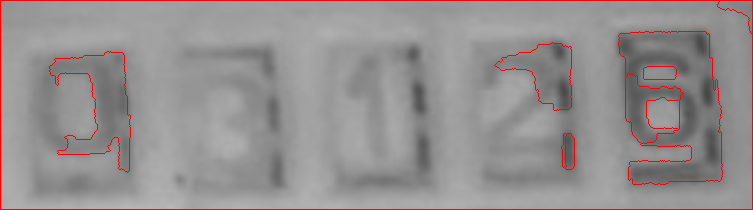
\includegraphics[width=0.9\linewidth]{../assets/watershed.png}\\{\scriptsize watershed boundaries (red)}
    \end{center}\end{column}
  \end{columns}
  \vspace{3pt}
  The distance transform peaks at each object's centre; watershed ``floods'' from those peaks and
  builds a ridge where floods meet --- the separating boundary.
\end{frame}

\begin{frame}{Distance transform --- worked}
  Distance-to-nearest-background of the touching blob from before:
  \begin{center}
  \pixelgrid{ {0,1,1,1,1,0}, {0,1,2,2,1,0}, {0,1,1,1,1,0} }
  \end{center}
  \begin{itemize}
    \item Each foreground pixel gets its distance to the nearest 0.
    \item \alert{Two peaks} appear (value 2) --- one per digit centre --- even though the
          shapes touch.
    \item Those peaks become the watershed \term{markers}: two basins, so two objects.
  \end{itemize}
\end{frame}

\begin{frame}{Watershed intuition}
  \begin{columns}[T]
    \begin{column}{0.46\textwidth}
      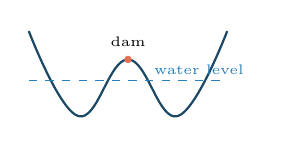
\begin{tikzpicture}[scale=0.9]
        \draw[coursePrimary,thick] plot[smooth,tension=0.7] coordinates
          {(0,1.4)(0.7,0.2)(1.4,1.0)(2.1,0.2)(2.8,1.4)};
        \draw[courseInfo,dashed] (0,0.7)--(2.8,0.7);
        \node[font=\tiny,courseInfo] at (2.4,0.85){water level};
        \fill[courseAccent] (1.4,1.0) circle (1.5pt);
        \node[font=\tiny] at (1.4,1.25){dam};
      \end{tikzpicture}
    \end{column}
    \begin{column}{0.54\textwidth}
      \begin{itemize}
        \item Treat intensity (or $-$distance) as a landscape; ``water'' rises from marked minima.
        \item Where two catchment basins meet, build a dam --- that dam is the object boundary.
        \item \term{Markers} (seeds) control it, or it \term{over-segments}.
      \end{itemize}
    \end{column}
  \end{columns}
\end{frame}

\begin{frame}{The over-segmentation trap}
  \begin{columns}[T]
    \begin{column}{0.5\textwidth}
      \begin{badbox}
        Raw watershed makes \emph{every} local minimum its own basin --- noise creates
        dozens of tiny bogus regions.
      \end{badbox}
    \end{column}
    \begin{column}{0.5\textwidth}
      \begin{goodbox}
        Marker-controlled watershed: flood only from \emph{chosen} markers
        (sure-foreground) and let everything else be decided by the ridges.
      \end{goodbox}
    \end{column}
  \end{columns}
  \keyidea{Never run watershed unseeded on a noisy image --- always give it markers.}
\end{frame}

\begin{frame}{Marker-controlled watershed --- the recipe}
  \begin{enumerate}
    \item Threshold to a clean binary (Session 1).
    \item Distance transform; its high peaks $=$ \term{sure foreground}.
    \item Dilate the binary $=$ \term{sure background}; the rest is \term{unknown}.
    \item Label the sure-foreground blobs (connected components) as markers.
    \item Run \code{cv2.watershed}; it assigns every unknown pixel and marks ridges $=-1$.
  \end{enumerate}
  \begin{goodbox}
    Threshold on the distance peak (e.g. $0.5\times$max) trades off: higher $\to$ fewer,
    surer markers; lower $\to$ risk of re-merging.
  \end{goodbox}
\end{frame}

\begin{frame}[fragile]{Watershed in code (marker-controlled)}
\begin{lstlisting}[language=Python]
dist = cv2.distanceTransform(binary, cv2.DIST_L2, 5)
_, sure_fg = cv2.threshold(dist, 0.5*dist.max(), 255, 0)  # digit centres
sure_bg = cv2.dilate(binary, k, iterations=3)
unknown = cv2.subtract(sure_bg, np.uint8(sure_fg))
_, markers = cv2.connectedComponents(np.uint8(sure_fg))
markers = markers + 1; markers[unknown==255] = 0
markers = cv2.watershed(color_img, markers)               # -1 = boundaries
\end{lstlisting}
  \begin{itemize}
    \item \code{markers+1} keeps background $=1$; unknown set to $0$ for watershed to fill.
  \end{itemize}
\end{frame}

\begin{frame}{Watershed pitfalls}
  \begin{itemize}
    \item Peak threshold too high $\to$ a real digit gets no marker and merges with a neighbour.
    \item Peak threshold too low $\to$ one digit sprouts two markers and splits.
    \item Forgetting to pass the \emph{colour} image to \code{cv2.watershed} (it needs 3 channels).
  \end{itemize}
  \begin{badbox}
    The $-1$ ridge pixels belong to \emph{no} object --- remember to ignore or reassign
    them before measuring areas.
  \end{badbox}
\end{frame}

% ==================================================================
\section{Connected components}
% ==================================================================

\begin{frame}{Labelling separate blobs}
  \begin{columns}[T]
    \begin{column}{0.55\textwidth}\begin{center}
      
\includegraphics[width=0.95\linewidth]{../assets/components.png}\\{\scriptsize each blob a different colour}
    \end{center}\end{column}
    \begin{column}{0.45\textwidth}
      \begin{itemize}
        \item \term{Connected components} labels each separate white region with an integer.
        \item Once separated, each digit is its own component you can crop and read (Week 13).
        \item \code{cv2.connectedComponents} / \code{...WithStats} give labels + areas + boxes.
      \end{itemize}
    \end{column}
  \end{columns}
\end{frame}

\begin{frame}{4- vs 8-connectivity}
  \begin{columns}[T]
    \begin{column}{0.5\textwidth}
      \begin{center}
      \pixelgrid{ {1,0,0}, {0,1,0}, {0,0,1} }
      \end{center}
    \end{column}
    \begin{column}{0.5\textwidth}
      \begin{itemize}
        \item \term{4-connectivity}: only up/down/left/right $\to$ 3 separate components.
        \item \term{8-connectivity}: diagonals count $\to$ 1 component.
        \item The choice changes counts --- pick it deliberately.
      \end{itemize}
    \end{column}
  \end{columns}
  \begin{badbox}
    A diagonal ``bridge'' of noise can fuse two digits under 8-connectivity. For separated
    digits, 4-connectivity is often safer.
  \end{badbox}
\end{frame}

\begin{frame}{Two-pass labelling (classic algorithm)}
  \begin{enumerate}
    \item \textbf{Pass 1:} scan row-major; give each foreground pixel the smallest label
          among its already-seen neighbours (or a new label). Record label equivalences.
    \item \textbf{Resolve:} union-find collapses equivalent labels to one representative.
    \item \textbf{Pass 2:} relabel every pixel with its representative.
  \end{enumerate}
  \begin{infobox}
    OpenCV's \code{connectedComponents} does this for you in $O(N)$; knowing the two
    passes explains why label numbers are not contiguous before resolution.
  \end{infobox}
\end{frame}

\begin{frame}[fragile]{Components with stats --- crop each digit}
\begin{lstlisting}[language=Python]
n, labels, stats, cents = cv2.connectedComponentsWithStats(
        binary, connectivity=8)
digits = []
for i in range(1, n):                       # 0 is background
    x, y, w, h, area = stats[i]
    if area < 40:                           # drop specks
        continue
    digits.append(binary[y:y+h, x:x+w])     # one cropped digit
digits.sort(key=lambda d: d.shape)          # (then order by x)
\end{lstlisting}
  \begin{itemize}
    \item \code{stats} gives x, y, w, h, area per label; \code{cents} the centroids.
  \end{itemize}
\end{frame}

\begin{frame}{Filtering \& ordering components}
  \begin{itemize}
    \item \term{Area filter}: drop components below a minimum area (noise) or above a
          maximum (the page border).
    \item \term{Aspect / fill}: a digit has a plausible height:width and fill ratio; use it
          to reject smudges.
    \item \term{Order}: sort surviving boxes by their $x$-centroid so digits read left-to-right.
  \end{itemize}
  \begin{goodbox}
    Sorting by $x$ (not by label id) is what makes ``42'' come out as \code{4},\code{2}
    and never \code{2},\code{4}.
  \end{goodbox}
\end{frame}

% ==================================================================
\section{Evaluating a segmentation}
% ==================================================================

\begin{frame}{Evaluating a segmentation}
  \begin{itemize}
    \item With ground-truth masks: \term{IoU} (intersection over union) and \term{Dice} score.
    \item Over-segmentation (too many regions) vs under-segmentation (merged regions) --- both are errors.
    \item For DocScan: the real test is downstream --- can each digit be read after segmentation?
  \end{itemize}
  \begin{mathbox}
    $\mathrm{IoU}=\dfrac{|A\cap B|}{|A\cup B|}$, \quad
    $\mathrm{Dice}=\dfrac{2|A\cap B|}{|A|+|B|}$ --- both are $1.0$ at perfect overlap.
  \end{mathbox}
\end{frame}

\begin{frame}{IoU --- a worked example}
  \begin{columns}[T]
    \begin{column}{0.4\textwidth}
      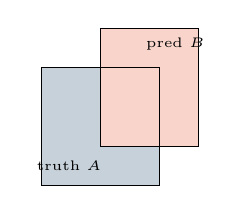
\begin{tikzpicture}[scale=0.5]
        \fill[coursePrimary!25] (0,0) rectangle (3,3);
        \fill[courseAccent!30] (1.5,1) rectangle (4,4);
        \draw (0,0) rectangle (3,3);
        \draw (1.5,1) rectangle (4,4);
        \node[font=\tiny] at (0.7,0.5){truth $A$};
        \node[font=\tiny] at (3.4,3.6){pred $B$};
      \end{tikzpicture}
    \end{column}
    \begin{column}{0.6\textwidth}
      Truth $A=3\times3=9$, pred $B=2.5\times3=7.5$, overlap $=1.5\times2=3$:
      \begin{mathbox}
        $\mathrm{IoU}=\dfrac{3}{9+7.5-3}=\dfrac{3}{13.5}=\alert{0.22}$\\[3pt]
        $\mathrm{Dice}=\dfrac{2\cdot3}{9+7.5}=\dfrac{6}{16.5}=0.36$
      \end{mathbox}
      Dice is always $\ge$ IoU for the same masks.
    \end{column}
  \end{columns}
\end{frame}

\begin{frame}{Over- vs under-segmentation}
  \begin{columns}[T]
    \begin{column}{0.5\textwidth}
      \begin{badbox}[Under-segmentation]
        Two digits share one label. Downstream reads a single wrong ``digit.'' Cause:
        marker missing / peak threshold too high.
      \end{badbox}
    \end{column}
    \begin{column}{0.5\textwidth}
      \begin{badbox}[Over-segmentation]
        One digit split into two labels. Downstream reads a phantom extra digit. Cause:
        noise minima / peak threshold too low.
      \end{badbox}
    \end{column}
  \end{columns}
  \keyidea{Tune the distance-peak threshold to the count you expect: the right number of components is itself a segmentation check.}
\end{frame}

% ==================================================================
\section{Beyond classical}
% ==================================================================

\begin{frame}{Classical vs deep segmentation}
  \begin{itemize}
    \item Classical (threshold/watershed/k-means): fast, interpretable, no training --- great for clean, structured images.
    \item Deep (U-Net, Mask R-CNN, SAM): learns to segment complex scenes, but needs data/compute.
    \item For meters/documents, classical often suffices; deep shines on messy natural scenes (Week 13--14).
  \end{itemize}
\end{frame}

\begin{frame}{GrabCut \& graph-based methods (brief)}
  \begin{itemize}
    \item \term{GrabCut}: model foreground/background colour distributions and cut the graph optimally --- interactive object cutout.
    \item Graph-cut / normalized-cut view segmentation as partitioning a pixel graph.
    \item These bridge classical and modern; good to know they exist.
  \end{itemize}
  \begin{infobox}
    You draw one box around the object; GrabCut iterates colour models + graph cut to
    refine the boundary --- no per-pixel labelling by hand.
  \end{infobox}
\end{frame}

% ==================================================================
\section{DocScan pipeline}
% ==================================================================

\begin{frame}{The segmentation pipeline for DocScan}
  \begin{center}
  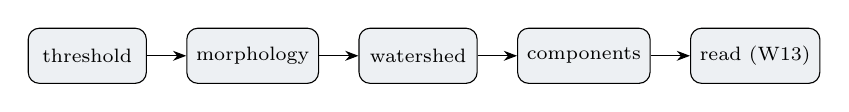
\begin{tikzpicture}[font=\scriptsize,>=Stealth,node distance=2mm and 5mm,
    b/.style={draw,rounded corners,fill=coursePrimary!8,minimum height=7mm,minimum width=15mm,align=center}]
    \node[b] (thr){threshold};
    \node[b,right=of thr] (mo){morphology};
    \node[b,right=of mo] (ws){watershed};
    \node[b,right=of ws] (cc){components};
    \node[b,right=of cc] (rd){read (W13)};
    \draw[->](thr)--(mo);\draw[->](mo)--(ws);\draw[->](ws)--(cc);\draw[->](cc)--(rd);
  \end{tikzpicture}
  \end{center}
  \begin{itemize}
    \item Threshold $\rightarrow$ clean $\rightarrow$ separate touching digits $\rightarrow$ label each $\rightarrow$ read.
    \item Each digit becomes an isolated image the CNN can classify.
  \end{itemize}
\end{frame}

\begin{frame}{Putting it together on the meter}
  \begin{enumerate}
    \item Adaptive threshold the meter crop (shadow-robust, Session 1).
    \item Morphological open to remove speckle (Week 7).
    \item Distance transform + marker-controlled watershed to split touching digits.
    \item \code{connectedComponentsWithStats}, area-filter, sort by $x$.
    \item Emit one cropped, ordered image per digit.
  \end{enumerate}
  \begin{goodbox}
    Validate by counting: if the meter shows 5 digits, your pipeline should output exactly
    5 components. Any other count flags a tuning problem.
  \end{goodbox}
\end{frame}

% ==================================================================
\section{Wrap-up}
% ==================================================================

\begin{frame}{What you should now be able to do}
  \begin{itemize}
    \item Separate touching objects with a marker-controlled watershed.
    \item Read a distance transform and place markers from its peaks.
    \item Label blobs with connected components; filter and order them.
    \item Evaluate a segmentation with IoU/Dice and diagnose over/under-segmentation.
  \end{itemize}
\end{frame}

\begin{frame}{This week's deliverable}
  \begin{alertblock}{Due before Week 9 (see \code{project/})}
    \begin{enumerate}
      \item Compare Otsu vs adaptive on meter images; pick the winner per lighting.
      \item k-means colour segmentation of a car/plate photo at $k=2,4,8$; discuss.
      \item Watershed to separate touching meter digits; label each with connected components.
      \item Report IoU/Dice against a hand-drawn mask for one image.
      \item DocScan milestone: output one cropped image per digit, in order.
    \end{enumerate}
  \end{alertblock}
\end{frame}

\begin{frame}[standout]
  Segmentation turns pixels into objects.\\[4pt]
  \normalsize Watershed separates touching shapes, components label them, IoU/Dice grade them.
\end{frame}

\end{document}
